
\documentclass[7x10,thmnumcontwithchapter,WebLink,AddlevelTwoTOC,NumRef,BookEndNote,printer]{pupbook}

\usepackage{makeidx}

\usepackage{graphicx}

%有限状态机
\usepackage{tikz}
\usetikzlibrary{automata, positioning, arrows}

\usepackage[ruled]{algorithm2e}

\usepackage{tikz-cd}

\usepackage{listings}
\usepackage{color}

\definecolor{dkgreen}{rgb}{0,0.6,0}
\definecolor{gray}{rgb}{0.5,0.5,0.5}
\definecolor{mauve}{rgb}{0.58,0,0.82}

\lstset{frame=tb,
	language=C++,
	aboveskip=3mm,
	belowskip=3mm,
	showstringspaces=false,
	columns=flexible,
	basicstyle={\small\ttfamily},
	numbers=none,
	numberstyle=\tiny\color{gray},
	keywordstyle=\color{blue},
	commentstyle=\color{dkgreen},
	stringstyle=\color{mauve},
	breaklines=true,
	breakatwhitespace=true,
	tabsize=3
}



%\usepackage{showframe}

\makeindex

\begin{document}

\frontmatter






\title{Category theory for Programmers\\ Solutions}



\author{littlekuo}



\makepuptitle

\cleardoublepage


\tableofcontents

\cleardoublepage

\mainmatter


\chapter[Category: The Essence of Composition]{Category: The Essence of Composition\thefootnote}


\begin{exercise}
~\\
Implement, as best as you can, the identity function in your favorite
language (or the second favorite, if your favorite language
happens to be Haskell).
\end{exercise}

\begin{proof}[Solution]
~\\
\begin{lstlisting}
auto id = [](auto x){ return x; }
\end{lstlisting}
\end{proof}


\begin{exercise}
	~\\
Implement the composition function in your favorite language. It
takes two functions as arguments and returns a function that is
their composition.
\end{exercise}

\begin{proof}[Solution]
	~\\
\begin{lstlisting}
auto compose = [](auto f, auto g) { 
 return [=](auto&& ... x) { 
    return f(g(x...)); 
 }; 
};
\end{lstlisting}
\end{proof}


\begin{exercise}
	~\\
Write a program that tries to test that your composition function
respects identity.
\end{exercise}

\begin{proof}[Solution]
~\\
\begin{lstlisting}
bool test_compose(){
  auto f = [](int str){
    return std::to_string(str);
  };
  auto f_id = compose(f, id);
  auto id_f = compose(id, f);
  for(int i = 0; i < 1000; i++){
    auto expect = f(i);
    auto r1 = f_id(i), r2 = id_f(i);
    if(r1 != expect || r2 != expect) 
       return false;
  }
    return true;
}
\end{lstlisting}
\end{proof}


\begin{exercise}
~\\
Is the world-wide web a category in any sense? Are links morphisms?
\end{exercise}

\begin{proof}[Solution]
If assume $A \rightarrow B$ is a morphism iff page B is reachable from page A in 0 or more steps, the world-wide web is a category.  \\
Links are not morphisms, because if there is a link on page A to page B, and a link on page B to page C, there not necessarily a link on page A to page C.
\end{proof}

\begin{exercise}
	~\\
	Is the world-wide web a category in any sense? Are links morphisms?
\end{exercise}

\begin{proof}[Solution]
	If assume $A \rightarrow B$ is a morphism iff page B is reachable from page A in 0 or more steps, the world-wide web is a category.  \\
	Links are not morphisms, because if there is a link on page A to page B, and a link on page B to page C, there not necessarily a link on page A to page C.
\end{proof}


\begin{exercise}
	~\\
Is Facebook a category, with people as objects and friendships as morphisms?
\end{exercise}

\begin{proof}[Solution]
It's not a category. Because if A and B are friends, and B and C are friends, A and C may not know each other.
\end{proof}


\chapter[Types and Functions]{Types and Functions\thefootnote}

\begin{exercise}
~\\
Define a higher-order function (or a function object) $memoize$ in
your favorite language. This function takes a pure function f as
an argument and returns a function that behaves almost exactly
like f, except that it only calls the original function once for every
argument, stores the result internally, and subsequently returns
this stored result every time it’s called with the same argument.
You can tell the memoized function from the original by watching
its performance. For instance, try to memoize a function that
takes a long time to evaluate. You’ll have to wait for the result
the first time you call it, but on subsequent calls, with the same
argument, you should get the result immediately.
\end{exercise}

\begin{proof}[Solution]
~\\
\begin{lstlisting}

template <typename T>
struct Memoize;

template<typename ResultType, typename... ArgTypes>
class Memoize<ResultType(ArgTypes...)>
{
private:
   using ArgsType = std::tuple<ArgTypes...>;
public:
   Memoize(std::function<ResultType(ArgTypes...)> f) : _f(f) {}

   ResultType operator()(ArgTypes... args) {
     const auto argsAsTuple = std::make_tuple(args...);
     auto memoized = _table.find(argsAsTuple);
     if(memoized == _table.end()) {
       auto const r = _f(args...);
       _table.insert({ {args...}, r});
       return r;
     } else {
       std::cout << "memoized: ->" << memoized->second << std::endl;
       return memoized->second;
     }
   }
private:
   std::map<ArgsType, ResultType> _table;
   std::function<ResultType(ArgTypes...)> _f;
};	
\end{lstlisting}
\end{proof}


\begin{exercise}
~\\
	Try to memoize a function from your standard library that you
	normally use to produce random numbers. Does it work?
\end{exercise}


\begin{proof}[Solution]
~\\
\begin{lstlisting}
auto memoizedRand = Memoize<int(void)>(rand);
std :: cout <<  memoizedRand() << std::endl;
std :: cout <<  memoizedRand() << std::endl;
\end{lstlisting}	
It always returns the same result. From the point of produce random numbers, it does not work.
\end{proof}


\begin{exercise}
	~\\
Most random number generators can be initialized with a seed.
Implement a function that takes a seed, calls the random number
generator with that seed, and returns the result. Memoize that
function. Does it work?
\end{exercise}

\begin{proof}[Solution]
	~\\
\begin{lstlisting}
int randNum(int seed){
   srand(seed);
   return rand();
}
auto memoizedRand = Memoize<int(int)>(randNum);

\end{lstlisting}	
this will always return the same random number for the same seed.
\end{proof}



\begin{exercise}
	~\\
Which of these C++ functions are pure? Try to memoize them
and observe what happens when you call them multiple times:
memoized and not. \\
(a) The factorial function from the example in the text. \\
(b) std::getchar() \\
(c)
\begin{lstlisting}
bool f() {
  std::cout << "Hello!" << std::endl;
  return true;
}
\end{lstlisting}
(d) 
\begin{lstlisting}
int f(int x) {
   static int y = 0;
   y += x;
   return y;
}
\end{lstlisting}
\end{exercise}

\begin{proof}[Solution]
~\\
(a) It is. there are only local variables, and return the same value when argument is the same. \\
(b) It is not pure. \\
(c) This function is not pure, since it outputs "Hello"(have side effects). \\
(d) It is not pure, because for the same argment, the return value may different.   
\end{proof}

\begin{exercise}
	How many different functions are there from Bool to Bool? Can
	you implement them all?
\end{exercise}


\begin{proof}[Solution]
~\\
\begin{lstlisting}
bool id(bool x){
  return x;
}

bool altrue(bool x){
  return true;
}

bool alfalse(bool x){
  return false;
}

bool neg(bool x){
  return !x;
}
\end{lstlisting}
\end{proof}

\begin{exercise}
Draw a picture of a category whose only objects are the types
$Void, () (unit), and Bool$; with arrows corresponding to all possible
functions between these types. Label the arrows with the
names of the functions
\end{exercise}


\begin{proof}[Solution]
~\\
\begin{figure}[ht]
	\centering 
		\scriptsize
		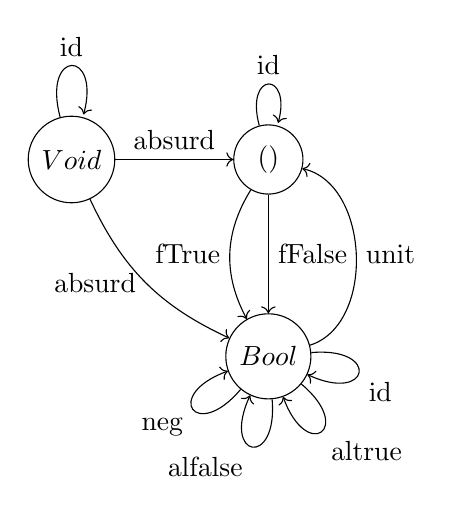
\begin{tikzpicture}[node distance=2.5cm, on grid, auto] 
		\node[state] (q_0)   {$Void$}; 
		\node[state] (q_1) [right=of q_0] {$( )$}; 
		\node[state] (q_2) [below=of q_1] {$Bool$}; 
		\path[->] 
		(q_0) edge  node {absurd} (q_1)
		(q_0) edge [bend right=20, left] node {absurd} (q_2)
		(q_0) edge [loop above] node {id} (q_1)
		
		(q_1) edge [loop above] node {id} (q_1)
		(q_1) edge [bend right = 30, left] node {fTrue} (q_2)
		(q_1) edge [] node {fFalse} (q_2)
		
		(q_2) edge [out=5,in=335,looseness=8] node {id} (q_2)
		(q_2) edge [out=320,in=290,looseness=8] node {altrue} (q_2)
		(q_2) edge [out=275,in=245,looseness=8] node {alfalse} (q_2)
	    (q_2) edge [out=230,in=200,looseness=8] node {neg} (q_2)
		
		(q_2) edge [bend right = 75, right] node {unit} (q_1)
		
		;
		\end{tikzpicture}
\end{figure} 
~\\
\end{proof}


\chapter[Categories Great and Small]{Categories Great and Small\thefootnote}

\begin{exercise}
Generate a free category from: \\
(a)A graph with one node and no edges \\
(b)A graph with one node and one (directed) edge (hint: this
edge can be composed with itself)\\
(c)A graph with two nodes and a single arrow between them \\
(d)A graph with a single node and 26 arrows marked with the letters of the alphabet: $a, b, c ... z$.
\end{exercise}


\begin{proof}[Solution]
~\\
(a) only one object and one morphism 
\begin{figure}[ht]
	\centering 
	\scriptsize
	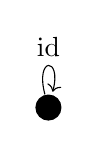
\begin{tikzpicture}[dot/.style={fill=black,circle,minimum size=2pt}] 
	\node[dot] (q_0)   {}; 
	\path[->] 
	(q_0) edge [loop above] node {id} (q_0)
	;
	\end{tikzpicture}
\end{figure} \\
(b) one object ; since the edge can be composed with itself, we may have infinitely many composed morphisms. 
\begin{figure}[ht]
	\centering 
	\scriptsize
	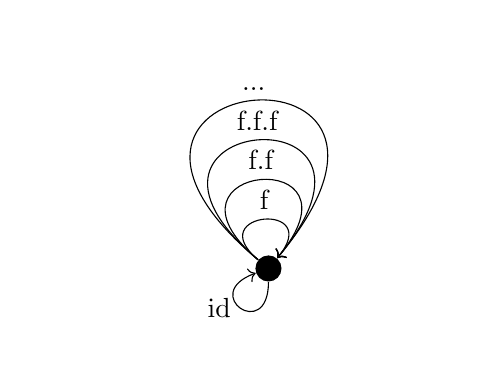
\begin{tikzpicture}[dot/.style={fill=black,circle,minimum size=2pt}] 
	\node[dot] (q_0)   {}; 
	\path[->] 
	(q_0) edge [out=270,in=200,looseness=10,left] node {id} (q_0)
	(q_0) edge [out=140,in=50,looseness=10,above] node {f} (q_0)
	(q_0) edge [out=140,in=50,looseness=20,above] node {f.f} (q_0)
	(q_0) edge [out=140,in=50,looseness=30,above] node {f.f.f} (q_0)
	(q_0) edge [out=140,in=50,looseness=40,above] node {...} (q_0)
	;
	\end{tikzpicture}
\end{figure} \\
(c) only one object and three morphisms.
\begin{figure}[ht]
	\centering 
	\scriptsize
	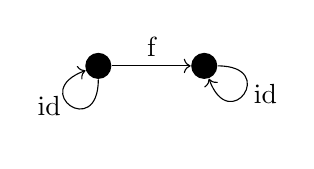
\begin{tikzpicture}[dot/.style={fill=black,circle,minimum size=2pt}] 
	\node[dot] (q_0)   {}; 
	\node[dot] (q_1) [right =of q_0]  {};
	\path[->] 
	(q_0) edge [out=270,in=200,looseness=10,left] node {id} (q_0)
	(q_1) edge [out=360,in=290,looseness=10,right] node {id} (q_1)
	(q_0) edge [above] node {f} (q_1)
	;
	\end{tikzpicture}
\end{figure} \\
(d) one object, similar to (b),  we may have infinitely many composed morphisms.
\begin{figure}[ht]
	\centering 
	\scriptsize
	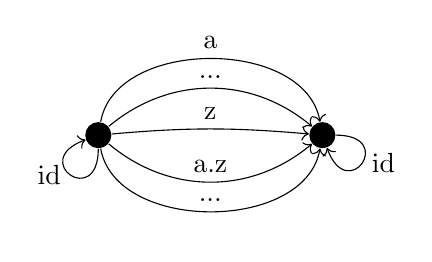
\begin{tikzpicture}[node distance=2.5cm, dot/.style={fill=black,circle,minimum size=2pt}] 
	\node[dot] (q_0)   {}; 
	\node[dot] (q_1) [right =of q_0]  {};
	\path[->] 
	(q_0) edge [out=270,in=200,looseness=10,left] node {id} (q_0)
	(q_1) edge [out=360,in=290,looseness=10,right] node {id} (q_1)
	(q_0) edge [bend left = 80, above] node {a} (q_1)
	(q_0) edge [bend left = 40, above] node {...} (q_1)
	(q_0) edge [bend left = 5,  above] node {z} (q_1)
	(q_0) edge [bend right = 40, above] node {a.z} (q_1)
	(q_0) edge [bend right = 80, above] node {...} (q_1)
	;
	\end{tikzpicture}
\end{figure} \\
\end{proof}


\begin{exercise}
What kind of order is this? \\
(a) A set of sets with the inclusion relation: $A$ is included in $B$ if every element of $A$ is also an element of $B$.\\
(b) C++ types with the following subtyping relation: $T1$ is a subtype of $T2$ if a pointer to $T1$ can be passed to a function that expects a pointer to $T2$ without triggering a compilation error.
\end{exercise}

\begin{proof}[Solution]
~\\
(a) Define $A \leq B$ as $A \subseteq B$. For every set $A$, $A \subseteq A$. $\subseteq$ is composable, $A \subseteq B$ and $B \subseteq C$ implies $A \subseteq C$. This means $\subseteq$ is a preorder. If $A \subseteq B $ and $B \subseteq A$ then $A = B$ which means it is a partial order. It is not a total order because $\{1\} \nsubseteq  \{2\}$ and $\{2\} \nsubseteq \{1\}$. \\
(b) Define $A \leq B$ as $A$ is  subtype  of  $B$. 	Similar to (a), it is at least a preorder.
\end{proof}


\begin{exercise}
Considering that $Bool$ is a set of two values $True$ and $False$, show
that it forms two (set-theoretical) monoids with respect to, respectively,
operator $\&\&$ (AND) and $||$ (OR).
\end{exercise}

\begin{proof}[Solution]
~\\
For operator $\&\&$,  $a \ \&\& \ (b \ \&\& \ c) = (a\ \&\& \ b) \ \&\& \ c$ (check eight cases),  so it is associative. The special element is
$True$. \\
For operator $||$, it is also associative. The special element is $False$. \\
\end{proof}



\begin{exercise}
Represent the $Bool$ monoid with the $AND$ operator as a category:
List the morphisms and their rules of composition.
\end{exercise}

\begin{proof}[Solution]
~\\
the morphsims are $True, False$,  the compositon of $f$, $g$ is $f \&\& g$.
\end{proof}


\begin{exercise}
Represent addition modulo 3 as a monoid category.
\end{exercise}

\begin{proof}[Solution]
~\\
the morphsims are $[0] , [1] , [2]$,  the compositon of $[a]$ and $[b]$ is $[(a+b) \ mod \ 3]$.
\end{proof}



\chapter[Kleisli Categories]{Kleisli Categories\thefootnote}

\begin{exercise}
Construct the Kleisli category for partial functions (define composition and identity).
\end{exercise}

\begin{proof}[Solution]
~\\
\begin{lstlisting}
template<class A, class B, class C> 
std::function<optional<C>(A)> compose(std::function<optional<C>(B)> m2,  std::function<optional<B>(A)> m1) {
     return [m1, m2](A x) {
       auto p1 = m1(x);
       if (!p1.isValid()) return optional<C>{};
       auto p2 = m2(p1.value());
       return p2;
     };
}
template<class A> optional<A> identity(A x) {
    return optional<A>{x};
}
\end{lstlisting}	
\end{proof}



\begin{exercise}
Implement the embellished function \textbf{safe\_reciprocal} that returns a valid reciprocal of its argument, if it’s different from zero.
\end{exercise}


\begin{proof}[Solution]
~\\
\begin{lstlisting}
optional<double> safe_reciprocal(double x) {
  if (x != 0) return optional<double>{1 / x};
  else return optional<double>{};
}
\end{lstlisting}
\end{proof}


\begin{exercise}
Compose the functions \textbf{safe\_root} and \textbf{safe\_reciprocal} to implement \textbf{safe\_root\_reciprocal} that calculates $sqrt(1/x)$ whenever possible.
\end{exercise}

\begin{proof}[Solution]
~\\
\begin{lstlisting}
optional<double> safe_root_reciprocal(double x) {
   return compose(safe_root, safe_reciprocal)(x);
}
\end{lstlisting}
\end{proof}


\chapter[Products and Coproducts]{Products and Coproducts\thefootnote}

\begin{exercise}
Show that the terminal object is unique up to unique isomorphism
\end{exercise}

\begin{proof}[Solution]
Suppose $A$ and $B$ are terminal objects, then there is exactly one morphism $f:A \rightarrow B$ and exactly one morphism $g: B \rightarrow A$(By definition of terminal object), So $fg: B \rightarrow B$ and  $gf: A \rightarrow A$, while $id_B: B \rightarrow B$ and  $id_A: A \rightarrow A$, we get $fg = id_B \ and \ gf = id_A$ (By definition of terminal object), thus any two terminal objects are isomorphic.
\end{proof}

\begin{exercise}
What is a product of two objects in a poset? Hint: Use the universal construction
\end{exercise}


\begin{proof}[Solution]
Suppose the product of two objecs $a, b$ is $c$  , we must have two projections:  
       $$ c \leq a \ and \  c \leq b $$
and for any other object $c'$ equipped with two projections:
       $$ c' \leq a \ and \  c' \leq b $$
then $c' \leq c$,  so the product of two objects in a poset is their greatest lower bound.
\end{proof}


\begin{exercise}
What is a coproduct of two objects in a poset?
\end{exercise}


\begin{proof}[Solution]
Suppose the product of two objecs $a, b$ is $c$  , we must have two injections:  
   $$ a \leq c \ and \  b \leq c $$
and for any other object $c'$ equipped with two projections:
   $$  a \leq c' \ and \  b \leq c' $$
then $c \leq c'$,  so the coproduct of two objects in a poset is their least upper bound.
\end{proof}


\begin{exercise}
Implement the equivalent of Haskell $Either$ as a generic type in your favorite language (other than Haskell).
\end{exercise}

\begin{proof}[Solution]
~\\
\begin{lstlisting}

\end{lstlisting}
\end{proof}


\begin{exercise}
	Show that $Either$ is a “better” coproduct than int equipped with two injections:
\begin{lstlisting}
int i(int n) { return n; }
int j(bool b) { return b ? 0: 1; }
\end{lstlisting}
Hint: Define a function
\begin{lstlisting}
int m(Either const & e);
\end{lstlisting}
that factorizes i and j.
\end{exercise}

\begin{proof}[Solution]
~\\	
\begin{lstlisting}
int m(Either const & e) {
 if (e.isLeft()) {
    return e.left;
 }
 return e.right?: 0; 1;
}
\end{lstlisting}
\end{proof}


\begin{exercise}
Continuing the previous problem: How would you argue that $int$ with the two injections i and j cannot be "better" than $Either$?
\end{exercise}

\begin{proof}[Solution]	
Suppose function
\begin{lstlisting}
Either m(int e);
\end{lstlisting}
factorizes function Left and Right. then
\begin{lstlisting}
Left = m.i
Right = m.j
\end{lstlisting}
So
\begin{lstlisting}
Left(0) = m(0);
Right(true) = m(0);
\end{lstlisting}
it means m(0) have different values which is impossible.
\end{proof}


\begin{exercise}
Still continuing: What about these injections?
\begin{lstlisting}
int i(int n) {
   if (n < 0) return n;
   return n + 2;
}
int j(bool b) { return b ? 0: 1; }
\end{lstlisting}
\end{exercise}


\begin{proof}[Solution]	
Define function
\begin{lstlisting}
Either m(int e) {
  if(e == 0){
     return Right(True);
  }
  if(e == 1){
     return Right(False);
  }
  if(e < 0){
     return  Left(e);
  }
  else {
     return Left(e-2);
  }
}
\end{lstlisting}
we can check $m . i = Left$ and $m . j = Right$.
\end{proof}


\begin{exercise}
Come up with an inferior candidate for a coproduct of $int$ and $bool$ that cannot be better than $Either$ because it allows multiple acceptable morphisms from it to $Either$.
\end{exercise}

\begin{proof}[Solution]
~\\
\begin{lstlisting}[language=Haskell]
data Tup = IntPair Int Int | BoolPair Bool Bool 

-- two injection
intToTup :: Int -> Tup;
intToTup x = IntPair x x

boolToTup :: Bool -> Tup;
boolToTup x = BoolPair x x 
\end{lstlisting}
Obviously there have many morphisms from it to Either 
\begin{lstlisting}[language=Haskell]
m :: Tup -> Either Int Bool;
m (IntPair x y) = if x == y then (Left x) else (Left 0) 
m (BoolPair x y) = if x == y then (Right x) else (Right False) 

m1 :: Tup -> Either Int Bool;
m1 (IntPair x y) = if x == y then (Left x) else (Left 1) 
m1 (BoolPair x y) = if x == y then (Right x) else (Right False)

m2 :: Tup -> Either Int Bool;
m2 (IntPair x y) = if x == y then (Left x) else (Left 3) 
m2 (BoolPair x y) = if x == y then (Right x) else (Right True)  
\end{lstlisting}
\end{proof}


\chapter[Simple Algebraic Data Types]{Simple Algebraic Data Types\thefootnote}

\begin{exercise}
Show the isomorphism between $Maybe \ a$ and $Either \ () \ a$.
\end{exercise}

\begin{proof}[Solution]
~\\	
\begin{lstlisting}[language=Haskell]
maybeToEither :: Maybe a -> Either () a
maybeToEither (Just a) = Right a
maybeToEither Nothing = Left ()

eitherToMaybe :: Either () a -> Maybe a
eitherToMaybe  (Right a) = Just a
eitherToMaybe  (Left ()) = Nothing
\end{lstlisting}
\end{proof}


\begin{exercise}
Here’s a sum type defined in Haskell: 
\begin{lstlisting}[language=Haskell]
data Shape = Circle Float | Rect Float Float
\end{lstlisting}

\end{exercise}



\end{document}
